\section{Fluid Mechanics}
\subsection{Kinematics}
\subsubsection{Coordinates}
\textbf{Lagrangian} $\underline{\boldmath{x}}(\underline{\boldmath{a}},t)$: The \textit{motion of individual particles} is studied; the position $\underline{\boldmath{x}}$ of a particle at time $t$ is related to its position at a reference point in time \underline{\boldmath{a}} (typically at $t=0$).
\newline
\newline
\textbf{Eulerian} $(\underline{\boldmath{x}},t)$: 
The \textit{'flow field' is considered as a whole} and the state of a fluid is described in terms of the values at a fixed location $\underline{\boldmath{x}}$ and at a fixed time $t$
\subsubsection{Velocity}
In Cartesian coordinates the velocity of a fluid particle at position $\underline{\boldmath{x}}(x,y,z)$ is given by:
\begin{center}
	$\underline{\boldmath{u}}(x,y,z) = u(x,y,z)\underline{\hat{i}} + v(x,y,z)\underline{\hat{j}} + w(x,y,z)\underline{\hat{k}}$
\end{center}
\subsubsection{Stagnation Points}
Stagnation points occur when the velocity vector $\underline{u}$ is equal to $\underline{0}$
\begin{align*}
	u = 0
	\\
	v= 0
	\\
	w= 0
\end{align*}
\subsubsection{Streamlines}
A streamline is a curve $C$ drawn at one point in time such that the fluid velocity vector $\underline{u}$ is tangent to $C$ at every point along $C$.
\begin{center}
	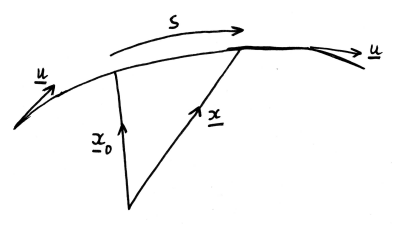
\includegraphics[width = 0.5\textwidth]{"Images/Streamline.png"}
\end{center} 
\begin{align*}
	\frac{d\underline{x}}{ds} = \underline{u}
	\\
	\\
	\frac{dx}{ds}=u , \frac{dy}{ds}=v ,  \frac{dz}{ds}=w
	\\
	\\
	\boxed{\frac{dx}{u}=\frac{dy}{v}=\frac{dz}{w}(= ds)}
\end{align*}

\subsubsection{Particle Paths}
Particle path is obtained by solving the initial value problem:
\begin{center}
		$\frac{d\underline{x}}{dt} = \underline{u}(\underline{x},t)$ , $\underline{x} = x_0$ at $t = 0$
		\\
		\begin{tabular}{|c|}
			\hline
			\\
				$\frac{dx}{dt} = u$ , $x(0)=x_0$
			\\ 
			\\
			$\frac{dy}{dt} = v$, $y(0)=y_0$
			\\
			\\
			$\frac{dz}{dt} = w$, $z(0)=z_0$
			\\
			\\
			\hline
		\end{tabular}
\end{center}

	
		


\subsubsection{Steady Flow}

\textbf{Steady Flow}: The flow velocity vector $\underline{u}$ is independent of time $t$
\newline
\textbf{Unsteady Flow}: $\underline{u}$ depends on $t$; the pattern of streamlines changes with $t$
\subsubsection{Convective Derivative}
The convective derivative tells us how a property changes \textit{as it moves with a flow}.
\\
\textbf{General}
\begin{center}
	\boxed{
		\frac{D\mathbf{*}}{Dt} =  \frac{\partial\mathbf{*}}{\partial t} + (\underline{u} \cdot \nabla)\mathbf{*}=\frac{\partial\mathbf{*}}{\partial t} + u\frac{\partial\mathbf{*}}{\partial x}+ v\frac{\partial\mathbf{*}}{\partial y} + w\frac{\partial\mathbf{*}}{\partial z}}
\end{center}
\textbf{Scalar}
\begin{center}
	\boxed{
		\frac{D\mathbf{\rho}}{Dt} =  \frac{\partial\mathbf{\rho}}{\partial t} + (\underline{u} \cdot \nabla)\mathbf{\rho} = \frac{\partial\mathbf{\rho}}{\partial t} + u\frac{\partial\mathbf{\rho}}{\partial x}+ v\frac{\partial\mathbf{\rho}}{\partial y} + w\frac{\partial\mathbf{\rho}}{\partial z}}
\end{center}
\textbf{Vector}
\begin{center}
	\boxed{
		\frac{D\mathbf{\underline{u}}}{Dt} =  \frac{\partial\mathbf{\underline{u}}}{\partial t} + (\underline{u} \cdot \nabla)\mathbf{\underline{u}}= \frac{\partial\mathbf{\underline{u}}}{\partial t} + u\frac{\partial\mathbf{\underline{u}}}{\partial x}+ v\frac{\partial\mathbf{\underline{u}}}{\partial y} + w\frac{\partial\mathbf{\underline{u}}}{\partial z}}
\end{center}
\subsubsection{Vorticity}
Vorticity \underline{$\omega$} is a measure of the local rotation of fluid particles in flow.
\\
\begin{center}
	\boxed{\underline{\omega} = \nabla \times \underline{u}}
\end{center}
\begin{center}
	$\nabla \times \underline{u} = \begin{vmatrix}
	\underline{i} & \underline{j} & \underline{k}\\ 
	\frac{\partial}{\partial x} & \frac{\partial}{\partial y} & \frac{\partial}{\partial z}\\
	u & v & w 
\end{vmatrix}$
\end{center}
\textbf{Irrotational Flow}:
\\
\begin{center}
	\boxed{\underline{\omega} = \underline{0}}
\end{center}
\subsubsection{Incompressible Flow}
\begin{center}
	\boxed{\nabla \cdot \underline{u} = 0}
\end{center}
	When this is true the convective derivative of the fluid density is zero:
	\begin{center}
		$\frac{D\rho}{Dt} = 0$
	\end{center}
\subsubsection{Velocity Potential}
For an irrotational flow the velocity can be described as the gradient of a scalar field known as the \textit{Velocity Potential}.
\begin{center}
	$\nabla \times \underline{u} = 0$
	\\
	The curl of the gradient of a scalar field is zero:
	\\
	$\nabla \times (\nabla \phi) = 0$
	\\
	$\underline{u} = \nabla\phi$
\end{center}
If the flow is also incompressible
\begin{center}
	$\nabla \cdot \underline{u} = 0$
	\\
	$\nabla \cdot (\nabla \phi) = 0$
	\\
	Therefore the velocity potential of an irrotational, incompressible flow satisfies Laplace's Equation:
	\\
	\boxed{\nabla^2 \phi = 0}
\end{center}
\subsubsection{Equipotential Surfaces}
Lines/surfaces of constant $\phi$ are \textit{equipotentials}.
\\
	The velocity potential can be considered a surface:
	\begin{center}
		$\phi(x,y,z)=c$
	\end{center}
	Let $\underline{a}$ be tangent to the surface, the derivative of $\phi$ in the direction of $\underline{a}$:
	\\
	\begin{center}
		$\underline{a}\cdot\nabla \phi = 0$
	\end{center}
	Because the derivative of a constant $c$ is zero: $\nabla \phi$ is normal to the surface.
	\begin{center}
		\boxed{\hat{\underline{n}}=\frac{\nabla \phi}{\vert\nabla \phi\vert} }
	\end{center}
\subsubsection{The Stream Function}
Considering incompressible two dimensional flow:
\begin{center}
	$\nabla \cdot \underline{u} = 0$
	\\
	$\frac{\partial u}{\partial x} + \frac{\partial v}{\partial y} = 0$	
\end{center}
We can introduce the stream function $\psi (x,y,t)$ such that:
\begin{center}
	\boxed{u = \frac{\partial \psi}{\partial y}, v=-\frac{\partial \psi}{\partial x}}
\end{center}
This satisfies the previous equations:
\begin{center}
	$\frac{\partial^2 \psi}{\partial x \partial y} - \frac{\partial^2 \psi}{\partial y \partial x} = 0$
\end{center}
\textbf{Vorticity of an incompressible two dimensional flow:}
\begin{center}
	$\underline{\omega} = \nabla \times \underline{u}$
	\\
	$\underline{\omega} = \frac{\partial v}{\partial x} - \frac{\partial u}{\partial y}$
	\\
	$\underline{\omega} = -\frac{\partial^2 \psi}{\partial^2 x} - \frac{\partial^2 \psi}{\partial^2 y}$
	\\
	\boxed{\underline{\omega}  = -\nabla^2\psi}
\end{center}

\subsection{Pressure in a Fluid}
\subsubsection{Pressure and Force}
Let the normal vector $\underline{n}$ be pointing into the fluid.
\begin{center}
	$\partial\underline{F} = -\partial F\underline{n}$
	\\
	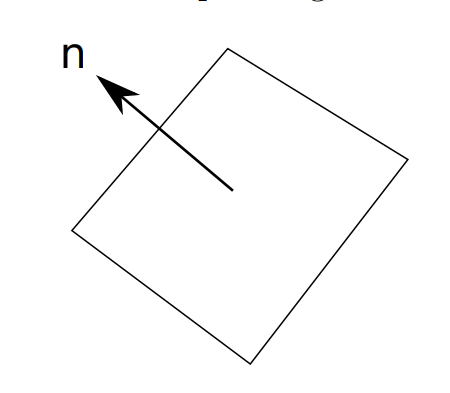
\includegraphics[width=0.3\textwidth]{Images/Pressure}
\end{center}
$\partial F$ is the force exerted over a small area $\partial S$
\\
\begin{center}
	$p = \lim \limits_{\partial S \to 0}(\frac{\partial F}{\partial S})$
	\\
	\boxed{\underline{F} = -\int \int_{S} p \underline{n} dS }
\end{center}
\subsubsection{Equations of State}
\textbf{Ideal Gas Law}
\\
\begin{center}
	$pV =nRT$
	\\
	$\frac{pV}{T} =  nR$
	\\
	$V \propto 1/\rho$
	\\
	\boxed{\frac{p}{\rho T} = constant}
\end{center}
\textbf{Isothermal Gas}
\\
For a gas at constant temperature $T$
\begin{center}
	Boyle's Law:
	\\
	$p \propto \rho$
	\\
	\boxed{p\rho^{-1}=p_{0}\rho_{0}^{-1}}
\end{center}
\textbf{Adiabatic Gas}
\\
 Quick fluctuations in pressure (such as in sound waves) are described by the adiabatic law.
 \begin{center}
 	\boxed{p\rho^{-\gamma} = c}
 \end{center}
Where $\gamma$ is the \textit{Polytropic Index}
\subsubsection{Hydrostatics}
\begin{center}
	The force due to the pressure of the fluid
	\\ 
	$\underline{F} = -\int \int_{S} p \underline{n} dS $
	\\
	Applying the divergence theorem for a scalar:
	\\
	$\underline{F} = - \int\int\int_V \nabla p dV$
	\\
	Calculating the weight of the fluid region:
	\\
	$\underline{W} = \int\int\int_V \rho \underline{g} dV$
	\\
	Since the fluid is stationary, the total force on the fluid is zero
	\\
	$\underline{W} + \underline{F} = 0$
	\\
	$\int\int\int_V \rho \underline{g} dV- \int\int\int_V \nabla p dV = 0$
	\\
	$\int\int\int_V (\rho \underline{g} - \nabla p) dV = 0$
	\\
	Therefore:
	\\
	\boxed{\rho \underline{g} = \nabla p}
	\\
	$\underline{g} = -g\hat{\underline{k}}$
	\\
	$\frac{\partial p}{\partial z} = -\rho g$
	\\
	Integrating gives:
	\\
	\boxed{p = p_a - \rho g z}
\end{center}
\subsubsection{Buoyancy}
Buoyancy is the force exerted on a submerged body due to the pressure of the surrounding static fluid.
\begin{center}
	$\underline{B} = -\int \int_{S} p \underline{n} dS$
	\\
	Applying the divergence theorem for a scalar:
	\\
	$\underline{B} = - \int\int\int_V \nabla p dV$
	\\
	$\nabla p = \rho \underline{g}$, $\underline{g} = -g\hat{\underline{k}}$
	\\
	$\underline{B} = \hat{\underline{k}} g \int \int \int_V \rho dV$
	\\
	\boxed{\underline{B} = \rho V g \hat{\underline{k}} = m_w g \hat{\underline{k}}}
\end{center}
\textbf{Archimedes’ Principle} – the buoyancy force on a body is equal in magnitude to the weight of fluid that is displaced by the body.
\begin{center}
	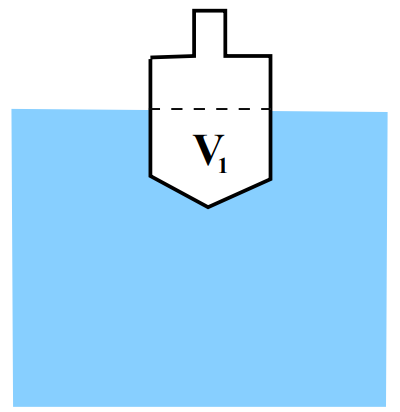
\includegraphics[width = 0.25\textwidth]{"Images/Buoyancy.png"}
	\\
	$V_1 = $ Volume od displaced water,\\
	$\rho_w = $ Density of water,\\
	$m_B = $ Mass of the body
	\\
	At equilibrium:
	\\
	$\underline{B} + \underline{W} = 0$
	\\
	$\rho_w V_1 g \hat{\underline{k}} - m_B g \hat{\underline{k}} = \underline{0}$
	\\
	\boxed{m_B = \rho_w V_1}
\end{center}
\textbf{Center of Mass (Gravity)}: A theoretical point in the body where the body’s total mass (weight) is thought to be concentrated.
\\
\textbf{Center of Buoyancy}: The centre of mass of the displaced water
\\
\newline
A floating body is stable if its centre of gravity is below its centre of buoyancy.
\subsubsection{Oscillation of a Floating Body}
When a floating body is submerged below its equilibrium depth $d$ it begins to oscillate.
\begin{center}
	Consider a cylindrical body with mass $m$, circular area $A$, equilibrium depth $d$:
	\newline
	\\
	$mz''(t) = \rho_w g (d-z(t))A- mg$
	\\
	$= - \rho_w g z(t)A$
	\\
	$= mg \frac{z(t)}{d}$
	\\
	Therefore you can form the differential equation:
	\\
	$z''(t)= \frac{g}{d}z(t)$
	\\
	$z(0) = -z_0$
	\\
	The solution:
	\\
	$z(t) = -z_0 \cos (\sqrt{\frac{g}{d}} t)$
\end{center}
\subsection{Flow Dynamics}
\subsubsection{Reynolds Transport Theorem}
\begin{tabular}{c}
	$\frac{d}{dt} \int_{\Omega(t)} F(\underline{x}, t) dV= \lim\limits_{\Delta t \to 0} [\int_{\Omega(t + \Delta t)} F(\underline{x},t+\Delta t) dV - \int_{\Omega(t)} F(\underline{x}, t)dV]$
	\\
	\\
	Using the Taylor series expansion:
	\\
	\\
	$\frac{d}{dt} \int_{\Omega(t)} F(\underline{x}, t) dV=\lim\limits_{\Delta t \to 0} [\int_{\Omega(t + \Delta t)} F(\underline{x}, t)+ \frac{\partial F}{\partial t}(\underline{x}, t)\Delta t + O(\Delta t)^2dV - \int_{\Omega(t)} F(\underline{x}, t)dV]$
	\\
	\\
	Let $\Delta \Omega$ be the difference between the regions $\Omega(t)$ and $\Omega(t + \Delta t)$:
	\\
	\\
	$\frac{d}{dt} \int_{\Omega(t)} F(\underline{x}, t) dV= \lim\limits_{\Delta t \to 0} [\int_{\Delta\Omega} F(\underline{x},t) dV + \int_{\Omega(t + \Delta t)} \frac{\partial F}{\partial t}(\underline{x}, t)\Delta t + O(\Delta t)^2dV]$
	\\
	\\
	Letting $U_n$ be the normal velocity to the boundary $\partial \Omega$
	\\
	\\
	$\frac{d}{dt} \int_{\Omega(t)} F(\underline{x}, t) dV= \lim\limits_{\Delta t \to 0} [\int_{\partial\Omega} F(\underline{x},t) U_n(\underline{x},t)\Delta t dS] + \lim\limits_{\Delta t \to \infty }[\int_{\Omega(t + \Delta t)} \frac{\partial F}{\partial t}(\underline{x}, t)\Delta tdV]$
	\\
	\\
	\boxed{\frac{d}{dt} \int_{\Omega(t)} F(\underline{x}, t) dV= \int_{\partial\Omega} F(\underline{x},t) U_n(\underline{x},t)dS + \int_{\Omega(t)} \frac{\partial F}{\partial t}(\underline{x}, t)dV}
\end{tabular}
\newline
\\
\textbf{Leibniz's Integral Rule}: The rule can be derived from considering a one dimensional case of \textit{Reynold's Transport Theorem}. 
\begin{center}
	\boxed{\frac{d}{dt}\int^{b(t)}_{a(t)} F(\underline{x},t) dx = \int^{b(t)}_{a(t)}\frac{\partial F}{\partial t}(\underline{x},t)dx + F(b(t),t)\frac{db}{dt} - F(a(t),t)\frac{da}{dt}}
\end{center}
\subsubsection{Conservation of Mass}
\subsection{Tow-dimensional Flow}
\subsection{Vorticity Dynamics}
\subsection{Free Surface Waves}